In this chapter are collected the results related to the most significant test cases. For each case all the combination of the setting used have given, together with the graph relative to the trend of the design variables, constraints and objective function until the iteration. The data relative to this trend are collected in a database, created using the recording function implemented in the openMDAO package. So to access to te result is required to use the openMDAO database function, for this reason an external component have been created in order to access to the database and plot the graphics.
\section{Reader code}
In order to collect all the information through the optimization process, the recorder function of openMDAO have been used. This function provide to create a database, which contain all the value of the variables. For each iteration a new dictionary will be created, this dictionary contain one dictionary for each type of variables, in the last there are all the value of the variables for that iteration, as showed in Fig. \ref{fig:6_1}:
\begin{figure}[H]
	\centering
	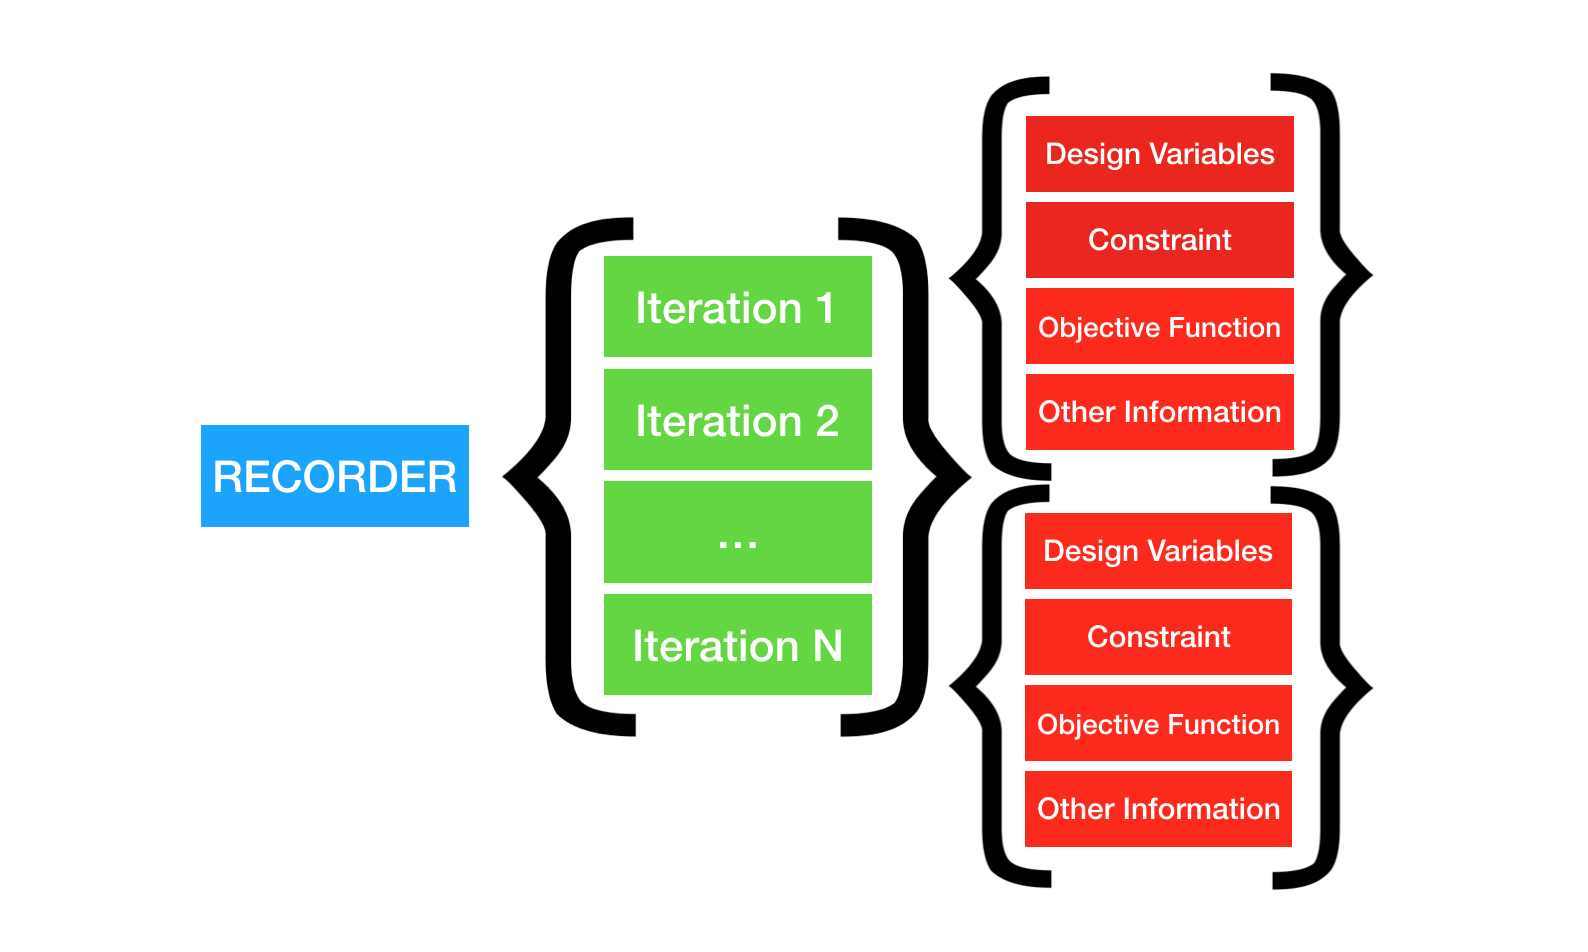
\includegraphics[width = 0.8\textwidth]{./Immagini/6_1.png}
	\caption{Structure of the recorder output file}
	\label{fig:6_1}
\end{figure}
Since the database file name is set, is possible to extract the keys of the dictionary, which are representative of the iterations. Depends on the optimization drives used, SLSQP or COBYLA, the extraction algorithm is different, so it's necessary to specify the used driver. Then for each iteration the value of the variables will be stored in a bunch of vector, defined by the user. At the end of the process a plotting section have been written in order to plot the trend of the variables. For the constraints plots also the limits of the constraint have been plotted, in order to see when a constraint is violated.\\
In Appendix A.2 is reported the python code written for extract the result, with indication of the function of each section.
\section{Test Cases Results}
In this section the result relative to the most significant test cases are given. For each case a table indicate all the setting parameters, while the results are stored in the output graph.
\subsection{Case 1}
In this test case an optimization of the CRM wing, full model, respect to the mass of the wing have performed. The driver chosen in this case is COBYLA, then the design limits have been implemented as constraint. The objective function is the mass of the wing, while the design variables are the angle of attack $\alpha$ and the thicknesses of the 12 shell element section of the structural model. The constraints are the lift constraint and the stress constraint, for the second the aggregation have been performed, using the $G_{KS}^L$ function. \\
In Fig. \ref{fig:6_2} are shown the trend of the variables until the optimization, for the stress are shown the maximum of Von Mises stress vector obtained using the maximum value function and the relative aggregation function value; for the aerodynamic variables the trend of the induced drag coefficient $C_{D_i}$ and the lift coefficient $C_L$ are shown. In Tab. \ref{tab:6_1} are summarised the information of the optimization settings.
\begin{table}[H]
	\centering
	\begin{tabular}{ccc}
		\hline
		\multicolumn{1}{|c|}{\textit{Options}}                          & \multicolumn{2}{c|}{\textit{Choice}}                                               \\ \hline
		\multicolumn{1}{|c|}{Wing Model}                       & \multicolumn{2}{c|}{CRM Wing}                                                     \\ \hline
		\multicolumn{1}{|c|}{Driver}                           & \multicolumn{2}{c|}{COBYLA}                                                     \\ \hline
		\multicolumn{1}{|c|}{Design Variable}                  & \multicolumn{1}{c|}{Angle of Attack}&\multicolumn{1}{c|}{Thicknesses}                                                     \\ \hline
				\multicolumn{1}{|c|}{Constraints}                  & \multicolumn{1}{c|}{Lift }&\multicolumn{1}{c|}{Stresses}                                                     \\ \hline
		\multicolumn{1}{|c|}{Objective Function}               & \multicolumn{2}{c|}{Mass}                                                     \\ \hline
		\multicolumn{1}{|c|}{\multirow{2}{*}{Generic Options}} & \multicolumn{1}{c|}{Constraints Aggregation}      & \multicolumn{1}{c|}{$\text{\rlap{$\checkmark$}}\square$} \\ \cline{2-3} 
		\multicolumn{1}{|c|}{}                                 & \multicolumn{1}{c|}{Design Limits as Constraints} & \multicolumn{1}{c|}{$\text{\rlap{$\checkmark$}}\square$} \\ \hline
		&                                                   &                      
	\end{tabular}
\caption{Optimization Settings Case 1}
\label{tab:6_1}
\end{table}
\begin{figure}[H]
	\centering
	\includegraphics[width = 1\textwidth]{./Immagini/Case1/opti_g_55_1.png}
\end{figure}
\begin{figure}[H]
	\centering
	\includegraphics[width = 1\textwidth]{./Immagini/Case1/opti_g_55_2.png}
\end{figure}
\begin{figure}[H]
	\centering
	\includegraphics[width = 0.8\textwidth]{./Immagini/Case1/opti_g_55_3.png}
	\caption{Result of the optimization Case 1}
	\label{fig:6_2}
\end{figure}
As you can see from the graph the optimization reach the convergence of the objective function in around 160 iteration. All the constraint are respected, and the optimization reach a gain in terms of structural mass of around 15\%, the initial mass of the wing was 17'200 Kg, at the end of the optimization the mass is around 15'000 Kg. As we can see using a lower bounded aggregation function the maximum of Von Mises stress exceed the limit. \\
For this optimization we use COBYLA, the gradien free optimization driver implemented. As we can see the driver choose the design direction for the optimization in an evaluation performed in the initial iteration, that we can see on the graph as a little step on the design variables. Once the direction it's decided he continue in that direction until the convergence. We can see how the direction is to reduce the thickness of the panel until the failure stress criteria allow it. The angle of attack is related to the $C_L$, so its initial value is chosen in order to respect the lift constraint. At iteration 40 the driver found the best design point, so from that point he start to evaluate the functions changing the design variable from that point, checking step by step the constraints.
\subsection{Case 2}
In this test case we have done an optimization on the CRM wing, in order to minimize the induced drag coefficient $C_{D_i}$ using, this time, the gradient based optimizer SLSQP, where, as we said, the gradient is computed using the finite difference method. The constraint are the lift constraint and the stress constraints, aggregate this time with the upper bounded Kreisselmeier-Steinhsauser function. This time, since COBYLA is not used, isn't necessary to set the design limits as constraint.\\
In Fig. \ref{fig:6_3} are showed the results, in the same format of the first case, while in Tab. \ref{tab:6_2} there are given the problem settings.
\begin{table}[H]
	\centering
	\begin{tabular}{ccc}
		\hline
		\multicolumn{1}{|c|}{\textit{Options}}                          & \multicolumn{2}{c|}{\textit{Choice}}                                               \\ \hline
		\multicolumn{1}{|c|}{Wing Model}                       & \multicolumn{2}{c|}{CRM Wing}                                                     \\ \hline
		\multicolumn{1}{|c|}{Driver}                           & \multicolumn{2}{c|}{SLSQP}                                                     \\ \hline
		\multicolumn{1}{|c|}{Design Variable}                  & \multicolumn{1}{c|}{Angle of Attack}&\multicolumn{1}{c|}{Thicknesses}                                                     \\ \hline
		\multicolumn{1}{|c|}{Constraints}                  & \multicolumn{1}{c|}{Lift }&\multicolumn{1}{c|}{Stresses}                                                     \\ \hline
		\multicolumn{1}{|c|}{Objective Function}               & \multicolumn{2}{c|}{Cdi}                                                     \\ \hline
		\multicolumn{1}{|c|}{\multirow{2}{*}{Generic Options}} & \multicolumn{1}{c|}{Constraints Aggregation}      & \multicolumn{1}{c|}{$\text{\rlap{$\checkmark$}}\square$} \\ \cline{2-3} 
		\multicolumn{1}{|c|}{}                                 & \multicolumn{1}{c|}{Design Limits as Constraints} & \multicolumn{1}{c|}{$\text{\rlap{$\xmark$}}\square$} \\ \hline
		&                                                   &                      
	\end{tabular}
	\caption{Optimization Settings Case 2}
	\label{tab:6_2}
\end{table}
\begin{figure}[H]
	\centering
	\includegraphics[width = 1\textwidth]{./Immagini/Case2/opti_g_36_1.png}
\end{figure}
\begin{figure}[H]
	\centering
	\includegraphics[width = 1\textwidth]{./Immagini/Case2/opti_g_36_2.png}
\end{figure}
\begin{figure}[H]
	\centering
	\includegraphics[width = 0.8\textwidth]{./Immagini/Case2/opti_g_36_3.png}
	\caption{Result of the optimization Case 2}
	\label{fig:6_3}
\end{figure}
In this case more than 220 iteration need to reach the convergence. The optimization target is the reduction of the induced drag coefficient, that see a reduction of the 25\%. No limits are imposed on the structural mass and on the minimum stress, so as we can see to reach this gain on the $C_{D_i}$ there is an increase of the mass of the 45\%, due to the increase of the thicknesses of the shell elements. This involves that the material is not fully exploited, the stresses are much lower than the yield stress. In this case we used an upper bounded aggregation function, so, as you can see, the value of the aggregation function is bigger than the value of the maximum of the Von Mises stress vector. Both the constraint are respected.\\
In this case we have used the gradient based optimizer, we can observe how the optimizer work, it start the initial condition, evaluate the gradient using the finite difference centered in that design point, than decide the direction of optimization and continue in that direction until the best condition are reached, then start a new gradient evaluation centered this time in the new design point, and it repeat this until the best is reached. So the graph are typed of strong excursions each time the gradient are computed. 
\subsection{Case 3 and 4}
The case 3 and 4 have the same settings, expect for the driver, in fact this test case have been done to got a comparison between the two different driver. In this cases the objective function is given by:
\begin{equation*}
f=\alpha C_{D_i}+ \beta m
\end{equation*}
where $\alpha = \beta = 0.5$, in order to obtain an optimization where the objective is find the best compromise between the mass and the induced drag, to avoid an optimization as the case 2 where to minimize the drag coefficient the mass of the wing grows disproportionately.\\
In Tab. \ref{tab:6_3} and Tab. \ref{tab:6_4} there are given respectively the setting option of the two case, while in Fig. \ref{fig:6_4} and Fig. \ref{fig:6_5} are showed the results graphs.
\begin{table}[H]
	\centering
	\begin{tabular}{ccc}
		\hline
		\multicolumn{1}{|c|}{\textit{Options}}                          & \multicolumn{2}{c|}{\textit{Choice}}                                               \\ \hline
		\multicolumn{1}{|c|}{Wing Model}                       & \multicolumn{2}{c|}{CRM Wing}                                                     \\ \hline
		\multicolumn{1}{|c|}{Driver}                           & \multicolumn{2}{c|}{SLSQP}                                                     \\ \hline
		\multicolumn{1}{|c|}{Design Variable}                  & \multicolumn{1}{c|}{Angle of Attack}&\multicolumn{1}{c|}{Thicknesses}                                                     \\ \hline
		\multicolumn{1}{|c|}{Constraints}                  & \multicolumn{1}{c|}{Lift }&\multicolumn{1}{c|}{Stresses}                                                     \\ \hline
		\multicolumn{1}{|c|}{Objective Function}               & \multicolumn{2}{c|}{$f= \alpha C_{D_i}+\beta m$}                                                     \\ \hline
		\multicolumn{1}{|c|}{\multirow{2}{*}{Generic Options}} & \multicolumn{1}{c|}{Constraints Aggregation}      & \multicolumn{1}{c|}{$\text{\rlap{$\checkmark$}}\square$} \\ \cline{2-3} 
		\multicolumn{1}{|c|}{}                                 & \multicolumn{1}{c|}{Design Limits as Constraints} & \multicolumn{1}{c|}{$\text{\rlap{$\xmark$}}\square$} \\ \hline
		&                                                   &                      
	\end{tabular}
	\caption{Optimization Settings Case 3}
	\label{tab:6_3}
\end{table}
\begin{figure}[H]
	\centering
	\includegraphics[width = 1\textwidth]{./Immagini/Case4/opti_g_33_1.png}
\end{figure}
\begin{figure}[H]
	\centering
	\includegraphics[width = 1\textwidth]{./Immagini/Case4/opti_g_33_2.png}
\end{figure}
\begin{figure}[H]
	\centering
	\includegraphics[width = 0.8\textwidth]{./Immagini/Case4/opti_g_33_3.png}
	\caption{Result of the optimization Case 3}
	\label{fig:6_4}
\end{figure}

\begin{table}[H]
	\centering
	\begin{tabular}{ccc}
		\hline
		\multicolumn{1}{|c|}{\textit{Options}}                          & \multicolumn{2}{c|}{\textit{Choice}}                                               \\ \hline
		\multicolumn{1}{|c|}{Wing Model}                       & \multicolumn{2}{c|}{CRM Wing}                                                     \\ \hline
		\multicolumn{1}{|c|}{Driver}                           & \multicolumn{2}{c|}{COBYLA}                                                     \\ \hline
		\multicolumn{1}{|c|}{Design Variable}                  & \multicolumn{1}{c|}{Angle of Attack}&\multicolumn{1}{c|}{Thicknesses}                                                     \\ \hline
		\multicolumn{1}{|c|}{Constraints}                  & \multicolumn{1}{c|}{Lift }&\multicolumn{1}{c|}{Stresses}                                                     \\ \hline
		\multicolumn{1}{|c|}{Objective Function}               & \multicolumn{2}{c|}{$f= \alpha C_{D_i}+\beta m$}                                                     \\ \hline
		\multicolumn{1}{|c|}{\multirow{2}{*}{Generic Options}} & \multicolumn{1}{c|}{Constraints Aggregation}      & \multicolumn{1}{c|}{$\text{\rlap{$\checkmark$}}\square$} \\ \cline{2-3} 
		\multicolumn{1}{|c|}{}                                 & \multicolumn{1}{c|}{Design Limits as Constraints} & \multicolumn{1}{c|}{$\text{\rlap{$\checkmark$}}\square$} \\ \hline
		&                                                   &                      
	\end{tabular}
	\caption{Optimization Settings Case 4}
	\label{tab:6_4}
\end{table}
\begin{figure}[H]
	\centering
	\includegraphics[width = 1\textwidth]{./Immagini/Case4/opti_g_50_1.png}
\end{figure}
\begin{figure}[H]
	\centering
	\includegraphics[width = 1\textwidth]{./Immagini/Case4/opti_g_50_2.png}
\end{figure}
\begin{figure}[H]
	\centering
	\includegraphics[width = 0.8\textwidth]{./Immagini/Case4/opti_g_50_3.png}
	\caption{Result of the optimization Case 4}
	\label{fig:6_5}
\end{figure}
The result of the objective functions, as expected, are in between of the result of the case 1 and case 2, which was polarized just on one objective function. In both cases in order to have a reduction of the induced drag coefficient it's necessary to increase the structural mass, but the increase is not bigger as the case 2.Though there are difference between the two optimization:

\begin{paracol}{2}
	\begin{leftcolumn*}
		\centering
		\textbf{COBYLA}
\begin{itemize}
	\item $\approx$200 iterations
	\item maximize the stresses
	\item final mass = + 11\%
	\item final $C_{D_i}$ = 0.037
\end{itemize}
	\end{leftcolumn*}
	\begin{rightcolumn}
		\centering
		\textbf{SLSQP}
		\begin{itemize}
			\item $\approx$ 220 iterations
			\item minimize $\alpha$
			\item final mass = + 27\%
			\item final $C_{D_i}$ = 0.039
				\end{itemize}
	\end{rightcolumn}
\end{paracol}
In Tab. \ref{tab:t5} a comparison of the important value of the optimization between the first 4 test case is given:
\begin{table}[H]
	\centering
	\begin{tabular}{|c|c|c|c|c|}
		\hline
		& Case 1 & Case 2 & Case 3 & Case 4 \\ \hline
		$\alpha \ [\deg]$ & 5.5    & 3.4    & 4.1    & 4.8    \\ \hline
		$C_L$             & 0.70   & 0.71   & 0.70   & 0.69   \\ \hline
		$C_{D_i}$         & 0.044  & 0.034  & 0.037  & 0.039  \\ \hline
		$m \ [Kg]$        & 14900  & 38000  & 23700  & 19600  \\ \hline
		
	\end{tabular}
	\caption{Comparison of Results}
	\label{tab:t5}
\end{table}
\subsection{Case 5}
This test case is relative to an optimization performed using the Goland wing, in order to obtain fast result in testing phase. Being the wing model different, the number of the section is different, but the structure of the script is the same. This optimization has as objective the function $f$, described in the test case 3 and 4, with $\alpha = \beta=1$.
\begin{table}[H]
	\centering
	\begin{tabular}{ccc}
		\hline
		\multicolumn{1}{|c|}{\textit{Options}}                          & \multicolumn{2}{c|}{\textit{Choice}}                                               \\ \hline
		\multicolumn{1}{|c|}{Wing Model}                       & \multicolumn{2}{c|}{Goland wing}                                                     \\ \hline
		\multicolumn{1}{|c|}{Driver}                           & \multicolumn{2}{c|}{COBYLA}                                                     \\ \hline
		\multicolumn{1}{|c|}{Design Variable}                  & \multicolumn{1}{c|}{Angle of Attack}&\multicolumn{1}{c|}{Thicknesses}                                                     \\ \hline
		\multicolumn{1}{|c|}{Constraints}                  & \multicolumn{1}{c|}{Lift }&\multicolumn{1}{c|}{Stresses}                                                     \\ \hline
		\multicolumn{1}{|c|}{Objective Function}               & \multicolumn{2}{c|}{$f= \alpha C_{D_i}+\beta m$}                                                     \\ \hline
		\multicolumn{1}{|c|}{\multirow{2}{*}{Generic Options}} & \multicolumn{1}{c|}{Constraints Aggregation}      & \multicolumn{1}{c|}{$\text{\rlap{$\xmark$}}\square$} \\ \cline{2-3} 
		\multicolumn{1}{|c|}{}                                 & \multicolumn{1}{c|}{Design Limits as Constraints} & \multicolumn{1}{c|}{$\text{\rlap{$\checkmark$}}\square$} \\ \hline
		&                                                   &                      
	\end{tabular}
	\caption{Optimization Settings Case 2}
	\label{tab:6_4}
\end{table}
\begin{figure}[H]
	\centering
	\includegraphics[width = 1\textwidth]{./Immagini/Case4/opti_g_20_1.png}
\end{figure}
\begin{figure}[H]
	\centering
	\includegraphics[width = 1\textwidth]{./Immagini/Case4/opti_g_20_2.png}
\end{figure}
\begin{figure}[H]
	\centering
	\includegraphics[width = 0.8\textwidth]{./Immagini/Case4/opti_g_20_3.png}
	\caption{Result of the optimization Case 5}
	\label{fig:6_6}
\end{figure}

